% Paper 2 (ICIMPACT 2027, sama dengan paper 1) — draf. Angka berasal dari angka.tex (dibuat angka.py dari cache).
% Aturan ICIMPACT: template konferensi IEEE, maks. 6 halaman termasuk referensi, review blind, tenggat EDAS 30 Nov 2026.
% \blindtrue = versi anonim untuk submisi; \blindfalse = versi bernama untuk camera-ready.
\newif\ifblind
\blindtrue
\documentclass[conference,a4paper]{IEEEtran}
\IEEEoverridecommandlockouts
\usepackage[utf8]{inputenc}
\usepackage[T1]{fontenc}
\usepackage{amsmath,amssymb}
\usepackage{graphicx}
\usepackage{booktabs}
\usepackage{array}
\usepackage{tabularx}
\usepackage{cite}
\usepackage[hidelinks]{hyperref}
% Dibuat otomatis oleh angka.py dari cache. Jangan diedit manual.
\newcommand{\nCfgAfdb}{12}
\newcommand{\nFam}{7}
\newcommand{\thrMin}{110}
\newcommand{\thrMax}{140}
\newcommand{\thrPtwo}{115}
\newcommand{\nSynth}{50}
\newcommand{\aflRegPtwo}{100}
\newcommand{\afGtwentyPtwo}{36}
\newcommand{\thrVsevenA}{135}
\newcommand{\thrVeightA}{120--140}
\newcommand{\nNormalAfdb}{99,000}
\newcommand{\nAfdbHi}{100}
\newcommand{\nAfdbHiPat}{7}
\newcommand{\pctAfdbHi}{0.1}
\newcommand{\cvAfdbHi}{0.18}
\newcommand{\cvAflHi}{0.03}
\newcommand{\afdbHiPtwo}{95}
\newcommand{\afdbHiMin}{72}
\newcommand{\afdbHiMax}{100}
\newcommand{\chapNhi}{1,743}
\newcommand{\chapNall}{6,797}
\newcommand{\chapPtwo}{99.2}
\newcommand{\chapPtwoCI}{[98.7, 99.5]}
\newcommand{\chapPkgMin}{98.9}
\newcommand{\chapPkgMax}{99.9}
\newcommand{\chapBandOne}{6}
\newcommand{\chapBandTwo}{55}
\newcommand{\chapVeightA}{25}
\newcommand{\chapVeightC}{20}
\newcommand{\nWinEx}{2,189}
\newcommand{\nSubjEx}{41}
\newcommand{\nSubjTotal}{52}
\newcommand{\nWinMan}{302}
\newcommand{\nSubjMan}{26}
\newcommand{\nPairWin}{192}
\newcommand{\nPairSubj}{24}
\newcommand{\nPairAlarmDev}{192}
\newcommand{\nPairAlarmRef}{192}
\newcommand{\exPtwo}{98.4}
\newcommand{\exPtwoCI}{[96.5, 99.6]}
\newcommand{\manPtwo}{100.0}
\newcommand{\nCfgEx}{6}
\newcommand{\exAfdbMin}{88.9}
\newcommand{\exAfdbMax}{99.9}
\newcommand{\manAfdbMin}{90.5}
\newcommand{\srcEpfl}{100}
\newcommand{\srcWrist}{100}
\newcommand{\srcEph}{98}
\newcommand{\exVsevenA}{63.9}
\newcommand{\dVsevenA}{$-$34.5}
\newcommand{\rVsevenA}{0.71}
\newcommand{\mfdVsevenA}{$-$0.006}
\newcommand{\mfpVsevenA}{0.41}
\newcommand{\exVsevenB}{70.9}
\newcommand{\dVsevenB}{$-$27.5}
\newcommand{\rVsevenB}{0.53}
\newcommand{\mfdVsevenB}{$-$0.131}
\newcommand{\mfpVsevenB}{0.00}
\newcommand{\exVeightA}{63.8}
\newcommand{\dVeightA}{$-$34.6}
\newcommand{\rVeightA}{0.00}
\newcommand{\mfdVeightA}{$-$0.115}
\newcommand{\mfpVeightA}{0.00}
\newcommand{\exVeightC}{60.3}
\newcommand{\dVeightC}{$-$38.1}
\newcommand{\rVeightC}{0.51}
\newcommand{\mfdVeightC}{$-$0.032}
\newcommand{\mfpVeightC}{0.23}
\newcommand{\rPtwo}{0.96}
\newcommand{\rPzero}{1.00}
\newcommand{\lolosDev}{68}
\newcommand{\lolosMan}{95}
\newcommand{\cvDev}{0.028}
\newcommand{\cvMan}{0.009}
\newcommand{\ltWristDev}{29}
\newcommand{\ltWristMan}{9}
\newcommand{\ltEphDev}{21}
\newcommand{\ruleMin}{61}
\newcommand{\ruleMax}{83}
\newcommand{\ruleManEpfl}{97}
\newcommand{\ruleAfl}{86}
\newcommand{\ruleAf}{0.2}
\newcommand{\ruleNormal}{0.1}
\newcommand{\abstRagu}{0}
\newcommand{\abstKosong}{12.9}
\newcommand{\abstAlarm}{86}
\newcommand{\abstNormal}{3.9}
\newcommand{\abstAfl}{9.7}
\newcommand{\aflShare}{58}
\newcommand{\tabelUtama}{
\multicolumn{7}{@{}l}{\textit{Trained on AFDB only}} \\
P0 MicroTransformer, original recipe & 110--115 & 94 & 98.9 & 98.0 [95.6, 99.5] & 100.0 & 1.00 \\
P1 MicroTransformer, fixed biases & 110--115 & 100 & 99.9 & 99.9 [99.7, 100.0] & 100.0 & 0.64 \\
P2 MicroTransformer, cross-fit biases (ref.) & 115 & 95 & 99.2 & 98.4 [96.5, 99.6] & 100.0 & 0.96 \\
BiGRU, soft weights & 120 & 87 & -- & 91.0 [87.4, 93.9] & 94.5 & 0.74 \\
BiGRU, full weights & 115--120 & 90 & -- & 96.0 [93.7, 97.7] & 98.4 & 1.00 \\
TCN, soft weights & 120--130 & 72 & -- & -- & -- & 0.01 \\
TCN, full weights & 120--125 & 84 & -- & 88.9 [85.0, 92.5] & 90.5 & 0.92 \\
InceptionTime, soft weights & 120--130 & 72 & -- & -- & -- & 0.79 \\
InceptionTime, full weights & 120--130 & 76 & -- & -- & -- & 0.99 \\
MiniRocket + logistic regression & 120--135 & 92 & -- & -- & -- & 0.11 \\
XGBoost (HRV features) & 115--125 & 85 & -- & -- & -- & 0.05 \\
RBF SVM (HRV features) & 120--140 & 78 & -- & -- & -- & 0.98 \\
\multicolumn{7}{@{}l}{\textit{Trained with sinus-tachycardia examples (MicroTransformer, soft weights)}} \\
+ synthetic ST, 100--130 bpm & 135 & 69 & -- & 63.9 [57.8, 70.0] & 65.1 & 0.71 \\
+ synthetic ST, 100--160 bpm & 85$^{a}$ & 86 & -- & 70.9 [66.5, 75.2] & 41.8 & 0.53 \\
+ Chapman (incl.\ clinical ST) & 120--140 & 81 & 25.5$^{b}$ & 63.8 [57.2, 71.1] & 32.4 & 0.00 \\
+ Chapman, AFL labels removed & 120--135 & 78 & 20.5$^{b}$ & 60.3 [53.3, 67.6] & 30.1 & 0.51 \\
}
\newcommand{\tabelMitigasi}{
Exercise $\geq$120\,bpm: alarm (\%) & 98.4 [96.5, 99.6] & 0.1 [0.0, 0.3] \\
Exercise $<$100\,bpm: alarm (\%) & 21.8 & 1.0 \\
Exercise: false alarms/h & 40.0 & 2.5 \\
\quad with 30\,s rule & 8.8 & 0.0 \\
PTB-XL sinus tach.\ ($n$=811): alarm (\%) & 29.7 & 1.6 \\
AFDB Normal 110--120\,bpm: alarm (\%) & 59.0 & 12.0 \\
AFDB sensitivity (window) & 0.934 & 0.893 \\
AFDB specificity (window) & 0.924 & 0.995 \\
AFDB episodes $\geq$30\,s found (30\,s rule) & 0.947 & 0.866 \\
AFDB false alarms/h (30\,s rule) & 1.59 & 0.08 \\
AFDB AFL windows ($n$=1,152): alarmed & 0.85 & 0.15 \\
\quad 08378, 2:1 flutter ($n$=306) & 1.00 & 0.00 \\
Icentia11k sensitivity (window) & 0.871 & 0.767 \\
}
\newcommand{\gateExHi}{0.1}
\newcommand{\gateExHiCiHi}{0.3}
\newcommand{\gateStach}{1.6}
\newcommand{\ptwoStach}{29.7}
\newcommand{\nStach}{811}
\newcommand{\ptwoExFa}{40.0}
\newcommand{\ptwoExFaRule}{8.8}
\newcommand{\gateExFaRule}{0.0}
\newcommand{\exHours}{30}
\newcommand{\exUnits}{52}
\newcommand{\gateSeDiff}{$-$0.040}
\newcommand{\gateSeDiffLo}{$-$0.086}
\newcommand{\gateSeDiffHi}{$-$0.002}
\newcommand{\gateSeDiffP}{0.02}
\newcommand{\gateIcentiaSe}{0.767}
\newcommand{\ptwoIcentiaSe}{0.871}
\newcommand{\nEightThreeAfl}{306}
\newcommand{\nAflAfdb}{1,152}
\newcommand{\gateEightThreeHit}{0}
\newcommand{\gateAflAll}{15}
\newcommand{\ptwoAflAll}{85}
\newcommand{\gateAfdbSe}{0.893}
\newcommand{\ptwoAfdbSe}{0.934}
\newcommand{\gateAfdbSp}{0.995}
\newcommand{\ptwoAfdbSp}{0.924}
\newcommand{\gateEpSe}{0.866}
\newcommand{\ptwoEpSe}{0.947}


\begin{document}
\bstctlcite{IEEEexample:BSTcontrol}

\title{Sinus Tachycardia Is a Blind Spot of RR-Interval Atrial Fibrillation and Flutter Classifiers Trained on the MIT-BIH
AFDB: A Stress Test with Synthetic, Clinical and Exercise ECG}

\ifblind
\author{\IEEEauthorblockN{Anonymous Author(s)}
\IEEEauthorblockA{Affiliation withheld for blind review}}
\else
\author{\IEEEauthorblockN{[Author 1], [Author 2], [Author 3], [Supervisor]}
\IEEEauthorblockA{\textit{[School / Faculty]}, \textit{Telkom University}, Bandung, Indonesia\\
\{[email]\}@[domain]}}
\fi

\maketitle

\begin{abstract}
The reference RR-interval classifier for atrial fibrillation (AF) and atrial flutter (AFL) raised an AF/AFL alarm on
\chapPtwo\% (95\% CI \chapPtwoCI) of \chapNhi{} physician-labelled sinus-tachycardia ECGs at $\geq$120\,bpm from the
Chapman--Shaoxing and Ningbo database. We stress-tested \nCfgAfdb{} configurations from \nFam{} model families trained on the
MIT-BIH Atrial Fibrillation Database (AFDB), where only \nAfdbHi{} of \nNormalAfdb{} Normal windows (\pctAfdbHi\%) reached
120\,bpm. On a synthetic regular-rhythm sweep (60--170\,bpm), the first heart rate at which fewer than half of the windows
were classified Normal ranged from \thrMin{} to \thrMax\,bpm. The reference alarmed on \exPtwo\% (95\% CI \exPtwoCI) of
\nWinEx{} exercise ECG windows at $\geq$120\,bpm from \nSubjEx{} volunteers using the 50\,Hz pipeline, and replacing detector
R-peaks with reference R-peaks did not remove the alarms (\nPairAlarmRef/\nPairWin{} matched windows).
Variants trained with synthetic or clinical sinus tachycardia lowered exercise alarm rates to \exVeightC--\exVsevenB\%, but
their recall of 2:1 flutter in AFDB record 08378 fell from \rPtwo{} to \rVeightA--\rVsevenA. In an exploratory analysis,
a zero-shot ECG foundation model used as a two-class gate on the same 50\,Hz windows alarmed on \gateExHi\% of these exercise
windows. Its AF/AFL sensitivity on AFDB was lower (\gateAfdbSe{} vs \ptwoAfdbSe), and it alarmed on
\gateEightThreeHit/\nEightThreeAfl{} 2:1 flutter windows in record 08378. Patient-wise AFDB evaluation cannot reveal this
failure mode, so RR-based AF/AFL studies should also report a synthetic regular-rhythm threshold and alarm rates on labelled
sinus tachycardia.
\end{abstract}

\begin{IEEEkeywords}
atrial fibrillation, atrial flutter, sinus tachycardia, RR interval, wearable ECG, stress test, distribution shift
\end{IEEEkeywords}

\section{Introduction}
Wearable single-lead ECG can screen for atrial fibrillation (AF) and atrial flutter (AFL) during daily life, and RR-interval
classifiers are attractive because beat detection fits low-power hardware sampling at 50\,Hz. Daily life includes exercise,
however, and exercise produces sinus tachycardia: a fast and regular rhythm. Fast regular RR sequences are also the signature of
AFL with 2:1 conduction, so an RR-only classifier must separate the two from rhythm timing alone.

The MIT-BIH Atrial Fibrillation Database (AFDB) is widely used to develop and evaluate RR-based
classifiers~\cite{moody1983afdb,goldberger2000physionet,pollard2026physionet}. Patient-wise evaluation on AFDB is known to be
fragile~\cite{butkuviene2021,domazetoski2022}. Sinus tachycardia caused false positives for an inter-beat-interval AF classifier
on wrist photoplethysmography~\cite{genzoni2020}, and deep models trained on PhysioNet/CinC 2017 AF data flagged 19--28\% of
118 sinus-tachycardia samples~\cite{sanjana2020}. Commercial ECG apps avoid the problem by design: they report a separate
high-heart-rate result from 100\,bpm and no rhythm classification above 140--150\,bpm~\cite{apple_ecg,fda_k240909,kardia}, and
their photoplethysmography notifications analyse data only while the user is still~\cite{fda_den180042,fda_k212372}. We found
no study that quantified how often AFDB-trained RR models alarm on sinus tachycardia, or whether AFDB-based evaluation can
detect it.

This paper reports a stress test of RR-interval AF/AFL classifiers developed for a 50\,Hz single-lead device, whose evaluation
protocol on AFDB is described elsewhere~\cite{anon_paper1}. We measure the first alarm threshold in a synthetic
regular-rhythm sweep and quantify how often AFDB contains windows in that heart-rate range. We test whether alarms occur on
physician-labelled sinus tachycardia and whether they persist when reference R-peaks are used on exercise ECG. We then
measure how training variants and post-hoc safeguards affect exercise alarm rates and 2:1 flutter recall in AFDB record 08378.
Finally, we explore whether an AF episode-duration rule and waveform information from a pretrained ECG model remove the
alarms, and what they cost.

\section{Methods}
\subsection{Models}
All models classify 10-s windows (up to 30 RR intervals and their differences) into Normal, AF and AFL. We trained \nCfgAfdb{} configurations
on AFDB only (23 records; windows from a beat detector run at 50\,Hz): three MicroTransformer recipes, namely the
original recipe with argmax decisions (P0), fixed decision biases (P1) and cross-fitted biases (P2, the deployed reference); BiGRU,
TCN and InceptionTime with soft (square-root) or full inverse-frequency class weights; MiniRocket with logistic regression; and
XGBoost and an RBF SVM on 16 HRV features. Four further MicroTransformer variants (soft class weights) were trained with
sinus-tachycardia examples: synthetic regular windows at 100--130 or 100--160\,bpm labelled Normal, or AFDB plus the
Chapman--Shaoxing and Ningbo databases~\cite{zheng2020chapman,zheng2020scirep,zheng2022ecgarrhythmia} (lead~II through the same front-end), either with all
labels or with AFL labels removed, because the Ningbo AFL labels had AF-like irregularity. AFDB metrics come from pooled
out-of-fold predictions in $5\times5$ patient-level cross-validation, averaged over repeats. For synthetic and exercise
tests, P0--P2 use their full-data packages, with a single fixed bias vector for P2. For other configurations we average
the window-level alarm indicators from the 25 fold models.

\subsection{Test sets}
\textit{AFDB by heart rate.} Out-of-fold predictions on AFDB Normal windows were grouped by mean heart rate. Normal
denotes the AFDB \texttt{(N} rhythm label.

\textit{Synthetic regular rhythms.} For 60--170\,bpm in 5-bpm steps we generated \nSynth{} windows per heart rate and
jitter type. The four types were constant RR intervals, uniform jitter ($\pm$10\,ms), and Gaussian jitter (SD 10 or
20\,ms). The alarm threshold is the first tested heart rate at which fewer than half of the windows are classified Normal.

\textit{Clinical sinus tachycardia.} From the PhysioNet version of Chapman--Shaoxing and Ningbo~\cite{zheng2022ecgarrhythmia} we
took the 10-s, 500-Hz ECGs labelled sinus tachycardia by physicians, processed lead~II with the 50\,Hz device front-end and kept
\chapNall{} recordings with a detected rate $\geq$100\,bpm (\chapNhi{} at $\geq$120\,bpm; one window per patient).

\textit{Exercise ECG.} Three public datasets were used: EPFL maximal cycling tests (20 subjects, 250\,Hz,
physician-reviewed R-peaks)~\cite{epfl_hi,degiovanni2023}, PhysioNet Wrist (8 volunteers walking, running and cycling, 256\,Hz
chest ECG with reference R-peaks)~\cite{jarchi2016wrist,physionet_wrist}, and EPHNOGRAM (24 healthy adults at rest, walking,
running and cycling, 8\,kHz)~\cite{kazemnejad2021ephnogram,kazemnejad2024}. Non-overlapping 10-s windows were built in two modes: \emph{device}, resampling to
50\,Hz, detecting beats and applying the production quality gate; and \emph{reference}, using the provided R-peaks (EPFL, Wrist).
In device mode, \nSubjEx{} of \nSubjTotal{} subjects contributed \nWinEx{} windows at $\geq$120\,bpm. The exercise datasets
provide ECG signals, with reference beat timing in EPFL and Wrist. For a paired P2 comparison we matched those windows
by dataset, subject, recording and start time, retaining windows that passed the quality gate and reached $\geq$120\,bpm
in both modes.

\subsection{Statistics and safeguards}
An alarm is a window classified AF or AFL. Exercise results use 2{,}000 subject-level bootstrap resamples for 95\% CIs and for
paired differences with P2. Clinical results for the packages use Wilson intervals. A rate-and-regularity rule flags
windows with rate $\geq$110\,bpm and RR coefficient of variation $\leq$0.05 for review. The conformal rule targets nominal
90\% coverage and reports uncertainty when the prediction set contains Normal and another class~\cite{angelopoulos2023}.
For AFDB evaluation we select the threshold across folds. For exercise evaluation we estimate the package threshold
from AFDB out-of-fold predictions with the package bias.

\subsection{Exploratory mitigation}
After the primary analysis we tested two additions that fit no parameter to our data. The \emph{episode rule} raises an alarm
only when consecutive AF/AFL windows span at least 30\,s, the minimum single-lead recording used to diagnose clinical
AF~\cite{vangelder2024esc}. A false alarm is an alarm episode that does not overlap a reference AF or AFL episode; exercise
recordings contain none, so every exercise alarm episode counts. The \emph{waveform gate} is the single-lead ECGFounder
model~\cite{li2025ecgfounder}, pretrained on over 10 million ECG recordings and applied zero-shot to the same 50\,Hz device
windows after upsampling to 500\,Hz and the model's own filtering. A window is alarmed when the softmax probability of its AF
plus AFL outputs exceeds that of its strongest sinus output (sinus rhythm, normal sinus rhythm or sinus tachycardia), with the
default threshold. The gate is a two-class detector and does not separate AF from AFL, so here an AFDB window counts as
detected if either system calls it AF or AFL. Both systems were also run on lead~I of the PTB-XL
recordings~\cite{wagner2020ptbxl} labelled sinus tachycardia and on Icentia11k wearable recordings~\cite{tan2019icentia},
through the same 50\,Hz front-end; P2 uses its full-data package there.

\section{Results}
\begin{table*}[t]
\centering
\caption{Sinus-tachycardia stress test. Alarm = window classified AF or AFL. Synthetic threshold: range over four jitter types.
Exercise rates use each mode's eligible windows, with 95\% subject-bootstrap CIs for device mode. Reference R-peaks are
available for EPFL and Wrist. The last column gives pooled out-of-fold AFL recall for record 08378 (2:1 flutter).
A dash marks an unevaluated configuration.}
\label{tab:main}
\footnotesize
\setlength{\tabcolsep}{3.2pt}
\begin{tabular}{@{}l c c c c c c@{}}
\toprule
& Synthetic & \multicolumn{4}{c}{Alarm rate at $\geq$120\,bpm (\%)} & AFDB AFL \\
\cmidrule(lr){3-6}
Configuration & threshold (bpm) & AFDB Normal & Clinical ST & Exercise, device & Exercise, reference & recall 08378 \\
\midrule
\tabelUtama
\bottomrule
\end{tabular}

\vspace{2pt}
\raggedright\footnotesize $^{a}$Non-monotonic: most regular windows at 85--90\,bpm were labelled AFL, Normal at 95--110\,bpm.
$^{b}$Chapman was part of training; cross-validated, not external.
\end{table*}

\subsection{Fast Normal windows are rare in AFDB}
Only \nAfdbHi{} of \nNormalAfdb{} AFDB Normal windows (\pctAfdbHi\%, \nAfdbHiPat{} patients) had a rate $\geq$120\,bpm, and they
were irregular (median RR coefficient of variation \cvAfdbHi{}, versus \cvAflHi{} for AFL windows $\geq$120\,bpm). AFDB-only
models alarmed on \afdbHiMin--\afdbHiMax\% of them (P2: \afdbHiPtwo\%; Table~\ref{tab:main}), but at this size the errors hardly
affect any AFDB metric.

\subsection{Synthetic sweep}
\begin{figure}[t]
\centering
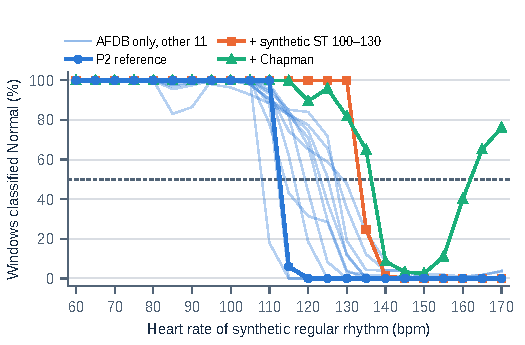
\includegraphics[width=\columnwidth]{gambar/sintetis.pdf}
\caption{Fraction of synthetic regular-rhythm windows (Gaussian RR jitter, SD 10\,ms) classified Normal. Thin lines: the other
AFDB-only configurations; the dashed line marks the 50\% threshold.}
\label{fig:synth}
\end{figure}

All \nCfgAfdb{} AFDB-only configurations crossed the 50\% threshold between \thrMin{} and \thrMax\,bpm (Fig.~\ref{fig:synth}).
P2 did so at \thrPtwo\,bpm for every jitter type. Perfectly regular windows $\geq$130\,bpm were classified AFL by P2 in
\aflRegPtwo\% of cases; with SD 20\,ms jitter, \afGtwentyPtwo\% became AF instead. Training with synthetic sinus tachycardia up
to 130\,bpm moved the threshold to \thrVsevenA\,bpm, just beyond the added range, and adding Chapman data moved it to
\thrVeightA\,bpm.

\subsection{Clinical sinus tachycardia and exercise ECG}
\begin{figure}[t]
\centering
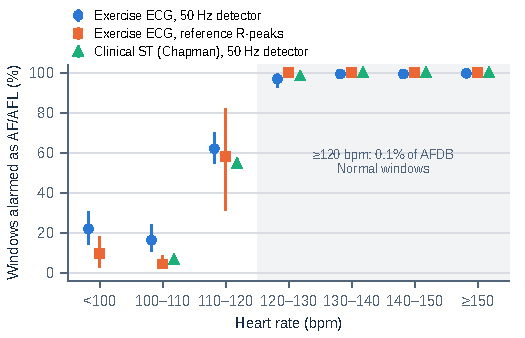
\includegraphics[width=\columnwidth]{gambar/pita.pdf}
\caption{Alarm rate of the reference model (P2) by heart rate on exercise ECG (device pipeline and reference R-peaks, 95\%
subject-bootstrap CIs) and on physician-labelled clinical sinus tachycardia. Shading marks rates rarely observed in
AFDB Normal windows.}
\label{fig:bands}
\end{figure}

The three packages alarmed on \chapPkgMin--\chapPkgMax\% of clinical sinus-tachycardia ECGs at $\geq$120\,bpm
(P2 \chapPtwo\%, 95\% CI \chapPtwoCI). In device mode, P2 alarmed on \exPtwo\% (95\% CI \exPtwoCI) of exercise
windows at $\geq$120\,bpm (EPFL \srcEpfl\%, Wrist \srcWrist\%, EPHNOGRAM \srcEph\%). Rates across the \nCfgEx{} AFDB-only
configurations tested on exercise ECG ranged from \exAfdbMin{} to \exAfdbMax\% (Table~\ref{tab:main}). Alarm rates rose
steeply across the heart-rate bands around 110--120\,bpm (Fig.~\ref{fig:bands}).

On the same \nPairWin{} EPFL and Wrist windows from \nPairSubj{} subjects, P2 alarmed on \nPairAlarmDev{}/\nPairWin{}
with detector R-peaks and \nPairAlarmRef{}/\nPairWin{} with reference R-peaks.

Across all \nWinMan{} eligible reference-mode windows (\nSubjMan{} subjects), P2 alarmed on \manPtwo\%, and AFDB-only
configurations alarmed on at least \manAfdbMin\%. On EPFL, \lolosDev\% of windows passed the quality
gate in device mode and \lolosMan\% passed with reference R-peaks. Median RR coefficient of variation was \cvDev{} in
device mode and \cvMan{} in reference mode. Below 100\,bpm, P2 alarmed on \ltWristDev\% of Wrist windows in device mode and
\ltWristMan\% in reference mode. The corresponding device-mode rate for EPHNOGRAM was \ltEphDev\%.

\subsection{Exercise alarm rates and 2:1 flutter recall}
\begin{figure}[t]
\centering
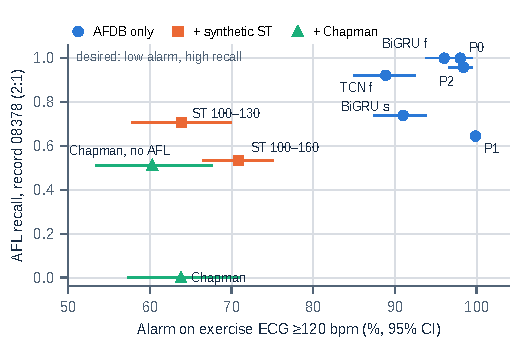
\includegraphics[width=\columnwidth]{gambar/tradeoff.pdf}
\caption{Exercise ECG alarm rate at $\geq$120\,bpm against 2:1 flutter recall for AFDB record 08378.
The figure includes configurations with exercise ECG predictions. The labels s and f denote soft and full class weights.}
\label{fig:tradeoff}
\end{figure}

The configurations trained with sinus-tachycardia examples had the lowest exercise alarm rates (Fig.~\ref{fig:tradeoff}).
The rate fell to \exVsevenA\% with synthetic examples up to 130\,bpm (\dVsevenA{} percentage points versus P2) and to
\exVeightC\% with Chapman data excluding AFL labels (\dVeightC{} points). Each variant had lower 2:1 flutter recall in record 08378
(recall \rPtwo{} for P2; \rVsevenA, \rVsevenB, \rVeightA{} and \rVeightC{} for the four variants), although the synthetic
100--130\,bpm variant was not distinguishable from P2 in AFDB macro-F1 ($\Delta$=\mfdVsevenA, $P$=\mfpVsevenA). Extending synthetic
examples to 160\,bpm made the model label regular rhythms at 85--90\,bpm as AFL (Table~\ref{tab:main}).

Conformal abstention marked \abstRagu\% of exercise ECG windows at $\geq$120\,bpm as uncertain. Counting empty prediction
sets as uncertain raised this to \abstKosong\% (alarms \abstAlarm\%) and made \abstNormal\% of Normal and \abstAfl\% of AFL
windows in AFDB uncertain.
The rate-and-regularity rule captured \ruleMin--\ruleMax\% of the exercise alarms in device mode (EPFL with reference R-peaks:
\ruleManEpfl\%), but on AFDB it also diverted \ruleAfl\% of correctly detected AFL, while touching only \ruleAf\% of AF windows.

\subsection{Exploratory mitigation}
\begin{table}[t]
\centering
\caption{Exploratory mitigation: P2 versus the zero-shot waveform gate (Gate) on the same windows. Alarm = AF or AFL. Exercise:
device mode; false alarms per hour of recording. AFDB: pooled out-of-fold predictions for P2.}
\label{tab:mitig}
\footnotesize
\setlength{\tabcolsep}{3pt}
\begin{tabular}{@{}l c c@{}}
\toprule
Measure & P2 & Gate \\
\midrule
\tabelMitigasi
\bottomrule
\end{tabular}
\end{table}

The episode rule alone did not remove the blind spot. Over \exHours{}\,h of exercise recordings from \exUnits{} subjects, P2
raised \ptwoExFa{} false alarm episodes per hour without the rule and \ptwoExFaRule{} with it (Table~\ref{tab:mitig}), because
sinus tachycardia during exercise is sustained. The waveform gate alarmed on \gateExHi\% of the \nWinEx{} exercise windows at
$\geq$120\,bpm (95\% CI upper bound \gateExHiCiHi\%) and on \gateStach\% of the \nStach{} PTB-XL sinus-tachycardia recordings
(P2: \ptwoStach\%); with the episode rule it raised no exercise alarm. The gate paid for this in sensitivity. On AFDB,
window sensitivity changed by \gateSeDiff{} (95\% CI [\gateSeDiffLo, \gateSeDiffHi]) while specificity rose from
\ptwoAfdbSp{} to \gateAfdbSp. The gate alarmed on \gateAflAll\% of the \nAflAfdb{} AFDB flutter windows (P2: \ptwoAflAll\%)
and on \gateEightThreeHit/\nEightThreeAfl{} 2:1 flutter windows in record 08378, calling them sinus. Its sensitivity
on Icentia11k was \gateIcentiaSe{} versus \ptwoIcentiaSe{} for P2.

\section{Discussion}
The synthetic alarm pattern appeared across all tested AFDB-only configurations. This is consistent with the composition
of AFDB, where fast Normal windows were scarce and had greater RR variability than fast AFL windows. Such sparse coverage
can leave high alarm rates at fast heart rates hidden in aggregate scores, even under patient-wise evaluation with
bootstrap confidence intervals~\cite{anon_paper1}. This extends earlier concerns about AFDB-based
evaluation~\cite{butkuviene2021,domazetoski2022} and complements reports of sinus-tachycardia false positives in an
inter-beat-interval classifier using photoplethysmography~\cite{genzoni2020}.

Sinus tachycardia and 2:1 flutter can have similar RR timing. The four training variants traded fewer exercise alarms for
lower 2:1 flutter recall in record 08378, and the rate-and-regularity rule diverted a large fraction of detected AFDB
flutter. The limited benefit of conformal abstention is consistent with distribution shift undermining the exchangeability
assumption~\cite{tibshirani2019,barber2023} and with conformal coverage losses reported for AI-ECG AF detection under
external deployment shift~\cite{abbasi2026}. A review flag for fast regular rhythms would need to be evaluated against both
outcomes.

A duration rule cannot help, because sinus tachycardia lasts as long as the exercise. The waveform gate removed nearly all
exercise alarms without any training on our data, whereas the RR variants trained with sinus-tachycardia examples still
alarmed on \exVeightC--\exVsevenB\% of exercise windows. This suggests that the ECG waveform carries most of the
information that separates sinus tachycardia from AF. The gate did not resolve the trade-off, however. Like the RR variants, it lost
the 2:1 flutter in record 08378, and it also lost sensitivity on wearable recordings. A two-class gate cannot report
flutter as a separate class either.

We recommend that RR-based AF/AFL evaluations report (i) the synthetic regular-rhythm threshold, (ii) the alarm rate on labelled
sinus tachycardia by heart-rate band, and (iii) results with the deployed beat detector during motion.

\textit{Limitations.} Exercise recordings lacked rhythm labels, so their alarm rates cannot establish a sinus-tachycardia
false-positive rate. Clinical sinus tachycardia came from resting 10-s ECGs in one database. Exercise results cover
\nCfgEx{} AFDB-only configurations. The paired analysis is restricted to EPFL and Wrist windows eligible in both modes.
The estimate of 2:1 flutter recall comes from a single AFDB record, and the synthetic rhythms omit respiratory and
autonomic dynamics. The mitigation analysis was added after the primary analysis, uses one pretrained model at its default
threshold and could not be run on the synthetic sweep, which has no ECG waveform.

\section{Conclusion}
At $\geq$120\,bpm, the three AFDB-trained packages alarmed on \chapPkgMin--\chapPkgMax\% of physician-labelled clinical
sinus-tachycardia ECGs. In the paired exercise analysis, alarms persisted with reference R-peaks. Training variants with
sinus-tachycardia examples lowered exercise alarm rates and reduced 2:1 flutter recall in AFDB record 08378.
A pretrained ECG waveform model used as a two-class gate nearly removed the exercise alarms, but its AF/AFL sensitivity was
lower and it detected none of the 2:1 flutter windows in record 08378. Evaluations for wearable use should include tachycardia stress tests and labelled device recordings.

\section*{Data and Code Availability}
All datasets are public (PhysioNet, Zenodo).
\ifblind
Code to reproduce all tables and figures from cached predictions will be released upon acceptance.
\else
[Code availability statement to be decided by the authors.]
\fi

\bibliographystyle{IEEEtran}
\bibliography{refs}

\end{document}
